% !TeX program = lualatex
\documentclass[final]{beamer}
% ====================
% Packages
% ====================
\usepackage{url}
\usepackage[T1]{fontenc}
\usepackage{lmodern}
\usepackage[orientation=portrait,size=a0,scale=1.00]{beamerposter}
\usetheme{gemini}
\usecolortheme{UBI}
\usepackage{graphicx}
\usepackage[portuguese]{babel}
\usepackage{pgfplots}
\pgfplotsset{compat=1.14}
\usepackage{anyfontsize}
\usepackage{xcolor}
\usepackage{adjustbox}
\usepackage{multicol}
\usepackage{siunitx}
\usepackage{caption}
\usepackage{url}
\usepackage{icomma}
\usepackage{tikz}
\usepackage{multicol}
\usepackage[most]{tcolorbox}
\definecolor{p1}{HTML}{caf0f8}
\definecolor{p2}{HTML}{ade8f4}
\definecolor{p3}{HTML}{90e0ef}
\definecolor{p4}{HTML}{48cae4}
\definecolor{p5}{HTML}{00b4d8}
\definecolor{p6}{HTML}{0096c7}
\definecolor{p7}{HTML}{0077b6}
\definecolor{p8}{HTML}{023e8a}
\definecolor{p9}{HTML}{03045e}
\definecolor{myred}{HTML}{f44336}
\definecolor{mypink}{HTML}{e81e63}
\definecolor{mypurple}{HTML}{9c27b0}
\definecolor{mydeeppurple}{HTML}{673ab7}
\definecolor{myindigo}{HTML}{3f51b5}
\definecolor{myblue}{HTML}{2196f3}
\definecolor{mylightblue}{HTML}{03a9f4}
\definecolor{mycyan}{HTML}{00bcd4}
\definecolor{myteal}{HTML}{009688}
\definecolor{mygreen}{HTML}{4caf50}
\definecolor{mylightgreen}{HTML}{8bc34a}
\definecolor{mylime}{HTML}{cddc39}
\definecolor{myyellow}{HTML}{ffeb3b}
\definecolor{myamber}{HTML}{ffc107}
\definecolor{myorange}{HTML}{ff9800}
\definecolor{mydeeporange}{HTML}{ff5722}
\definecolor{mybrown}{HTML}{795548}
\definecolor{mygray}{HTML}{9e9e9e}
\definecolor{mybluegray}{HTML}{607d8b}
\definecolor{pag}{HTML}{293133}
\definecolor{fundo}{RGB}{41, 49, 51}
\definecolor{UBI}{RGB}{12, 35, 64}
% ====================
% Lengths
% ====================
% If you have N columns, choose \sepwidth and \colwidth such that
% (N+1)*\sepwidth + N*\colwidth = \paperwidth
\newlength{\sepwidth}
\newlength{\colwidth}
\setlength{\sepwidth}{0.025\paperwidth}
\setlength{\colwidth}{0.45\paperwidth}
\newcommand{\separatorcolumn}{\begin{column}{\sepwidth}\end{column}}
% ====================
% Title
% ====================
\title{Queda de uma mola ideal suspensa com massas distribuídas regularmente}
\author{João Santos \inst{2} \and João Esteves \inst{2} \and José Amoreira \inst{1,2,3}}
\institute[]{\inst{1} Laboratório de Instrumentação e Física Experimental de Partículas \and  \inst{2}Universidade da Beira Interior  \samelineand \inst{3} Centro de Matemática e Aplicações (CMAUBI)}
% ====================
% Footer
% ====================
\footercontent{
  Física 2024 \hfill
%https://github.com/ljmamoreira/fslinky\hfill
  UBI - Departamento de Física}
% ====================
% Logos
% ====================
% use this to include logos on the left and/or right side of the header:
%\logoright{
\includegraphics[scale=1.5]{logos/DF2.png}}
\logoleft{
\includegraphics[scale=1.5]{logos/DF2.png}}
% ====================
% Corpo
% ====================
\begin{document}
\begin{frame}[t]
\begin{columns}[t]
\separatorcolumn
\begin{column}{\colwidth}
% -------------------------------
% Secção: Motivação/Introdução
% -------------------------------
\begin{exampleblock}{Motivação/Introdução}
  Vários vídeos disponíveis na plataforma YouTube mostram a queda de uma mola
  elástica a partir de uma situação de repouso estático em que ela se encontra
  na vertical, suspensa da sua extremidade superior. Estes vídeos são
  interessantes porque mostram a extremidade inferior da mola como que a aguardar
  que a extremidade superior a atinja, antes de começar o seu movimento de queda
  propriamente dito. 
	
  A explicação deste comportamento é dada pela teoria da elasticidade de um meio
  contínuo. A onda de deformação gerada na extremidade superior da mola quando é
  solta propaga-se longitudinalmente com uma velocidade finita, e só quando
  atinge a extremidade inferior, alterando aí o estado de deformação inicial, se
  modifica o equilíbrio de forças (peso e força elástica) que mantinham esta
  extremidade em repouso.
	
  Claramente, o modelo elementar de mola ideal, em que se despreza a sua massa,
  é insuficiente para enquadrar esta explicação, uma vez que não tendo massa,
  (1)~a sua deformação é sempre uniforme; logo, a força sobre a extremidade
  inferior altera-se instantaneamente assim que a extremidade superior inicia a
  sua queda, e (2)~a mola não fica sujeita à gravidade, ou seja, nem sequer cai!
  Mas será possível dar conta deste comportamento das molas reais considerando
  molas ideais com massas distribuídas regularmente ao longo do seu
  comprimento? Com este trabalho pretendeu-se dar resposta a esta questão.
\end{exampleblock}
% -------------------------------
% Secção: Formalismo
% -------------------------------
\begin{block}{Formalismo}
	\vspace{1cm}
	\newcommand{\mola}[4]%Quanto menor for o valor 3,4 e 5 dado à função mais comprimida estará a mola%
{
%------------------------------------------------------------Pontos Importantes------------------------------------------------------------%
\coordinate (bola1) at (0,{#1});
\coordinate (bola2) at (0,{#2}); 
\coordinate (bola3) at (0,-4);
\coordinate (bola4) at (0,-8);
\coordinate (reticencias) at (0,-6);
%-------------------------------------------------------------Desenhar as Molas------------------------------------------------------------%
\tikzstyle{spring}=[thick,decorate,decoration={aspect=.5, segment length=#3, amplitude=2.5mm,coil}]
\draw [spring] (bola2) -- (bola1);
\draw [spring] (bola3) -- (bola2);
\tikzstyle{spring}=[thick,decorate,decoration={aspect=.5, segment length=#4, amplitude=2.5mm,coil}]
\draw [spring] (bola4) -- (bola3);
%-------------------------------------------------------------Desenhar as Bolas------------------------------------------------------------%
\shade [ball color =white] (bola1) circle (.5) node[draw=none,inner sep = 0,scale=2,text=black]{};
\shade [ball color =white] (bola2) circle (.5) node[draw=none,inner sep = 0,scale=2,text=black]{};
\shade [ball color =white] (bola3) circle (.5) node[draw=none,inner sep = 0,scale=2,text=black]{};
\shade [ball color =white] (bola4) circle (.5) node[draw=none,inner sep = 0,scale=2,text=black]{};
%----------------------------------------------------------Desenhar as Reticências--------------------------------------------------------%
\node[rectangle,fill=white, minimum width = 2cm, minimum height = 1.1cm] (r) at (reticencias) {};
\draw (reticencias) node[ultra thick,scale=1,yshift=.05cm]{$\rotatebox{90}{$\cdots$}$} ;
}
\begin{minipage}{0.22\colwidth}
\resizebox{.2\colwidth}{!}{
\begin{tikzpicture}[scale=1, every node/.style={scale=.6}]
\mola{3}{-1.5}{3mm}{3mm}
\node[anchor=west] at (-1.5,3) {\textbf{\boldmath$1$}};
\node[anchor=west] at (-1.5,-1.5) {\textbf{\boldmath$2$}};
\node[anchor=west] at (-1.5,-4) {\textbf{\boldmath$3$}};
\node[anchor=west] at (-1.5,-8) {\textbf{\boldmath$N$}};
\draw[thick,->] (2,-8) -- (2,-6) node[draw=none,inner sep = 0,scale=1.5,xshift=.4cm,text=black]{$y$};
\end{tikzpicture}}
\end{minipage}
\begin{minipage}{0.7\colwidth}
Mola ideal com comprimento natural $L$ com constante elástica $K$, com $N$
partículas pontuais iguais com massa $m=M/N$, dispostas regularmente ao longo da
mola.
\begin{align*}
  l&=L/(N-1)&&\rightarrow\text{Comprimento de cada segmento}\\
  k&=K(N-1)&& \rightarrow\text{Constante elástica de cada segmento}\\
  m&=M/N    &&\rightarrow\text{Massa de cada partícula}
\end{align*}
Posições de equilíbrio iniciais:
\begin{equation*}
  %y_i^0=y_0^0-i\left[l+\left(N-\frac{i+1}{2}\right)\frac{mg}{k}\right],\quad i>0
  y_i^0=y_1^0-(i-1)\left[l+\left(N-\frac{i}{2}\right)\frac{mg}{k}\right],
  \quad i>1
\end{equation*}
Acelerações ($x_i=y_i-y_i^0$, $\omega^2=k/m$):
  \begin{align*}
    %\ddot x_0 &=-Ng+\omega^2(x_1-x_0)\\
    \ddot x_1 &=-Ng-\omega^2(x_1-x_2)\\
    \ddot x_i &= \omega^2(x_{i-1}-2x_i+x_{i+1}),\qquad i=2, \ldots, N-1\\
    %\ddot x_{N-1} &=\omega^2(x_{N-2}-x_{N-1})
    \ddot x_{N} &=\omega^2(x_{N-1}-x_{N})
  \end{align*}
\end{minipage}\\[1cm]
Este sistema de equações foi resolvido em Python/Numpy, usando a função
\texttt{solve\_ivp} da biblioteca SciPy.

\end{block}
% -------------------------------
% Secção: Procedimento experimental
% -------------------------------
\begin{block}{Procedimento experimental}
Para verificar a validade das soluções obtidas numericamente, estudou-se o
movimento de queda de uma mola de aço com bolas de ténis dispostas
regularmente ao longo do seu comprimento.  As bolas de ténis usadas têm massa
$56,6\pm0,1$\,g.  A massa da mola usada tem o valor $37,5\pm0,1$\,g;
determinou\-{-se} a sua constante elástica por regressão linear dos valores do
elongamento sob diferentes tensões, tendo-se obtido o valor de
$0,44\pm0,01$\,N/m.  O movimento de queda foi filmado a 120 fps e a posição das
bolas foi obtida fotograma a fotograma usando o programa Tracker \cite{Tracker}.
Analizaram-se os casos $N=2$ (uma massa em cada extremidade da mola) e $N=3$ (a
massa adicional no centro da mola). Os resultados estão apresentados na
Figura~\ref{fig:a}.

Verifica-se genericamente bom acordo entre os resultados numéricos e os valores
observados experimentalmente, o que valida o modelo.
\vspace{2cm}
\begin{center}
\begin{figure}
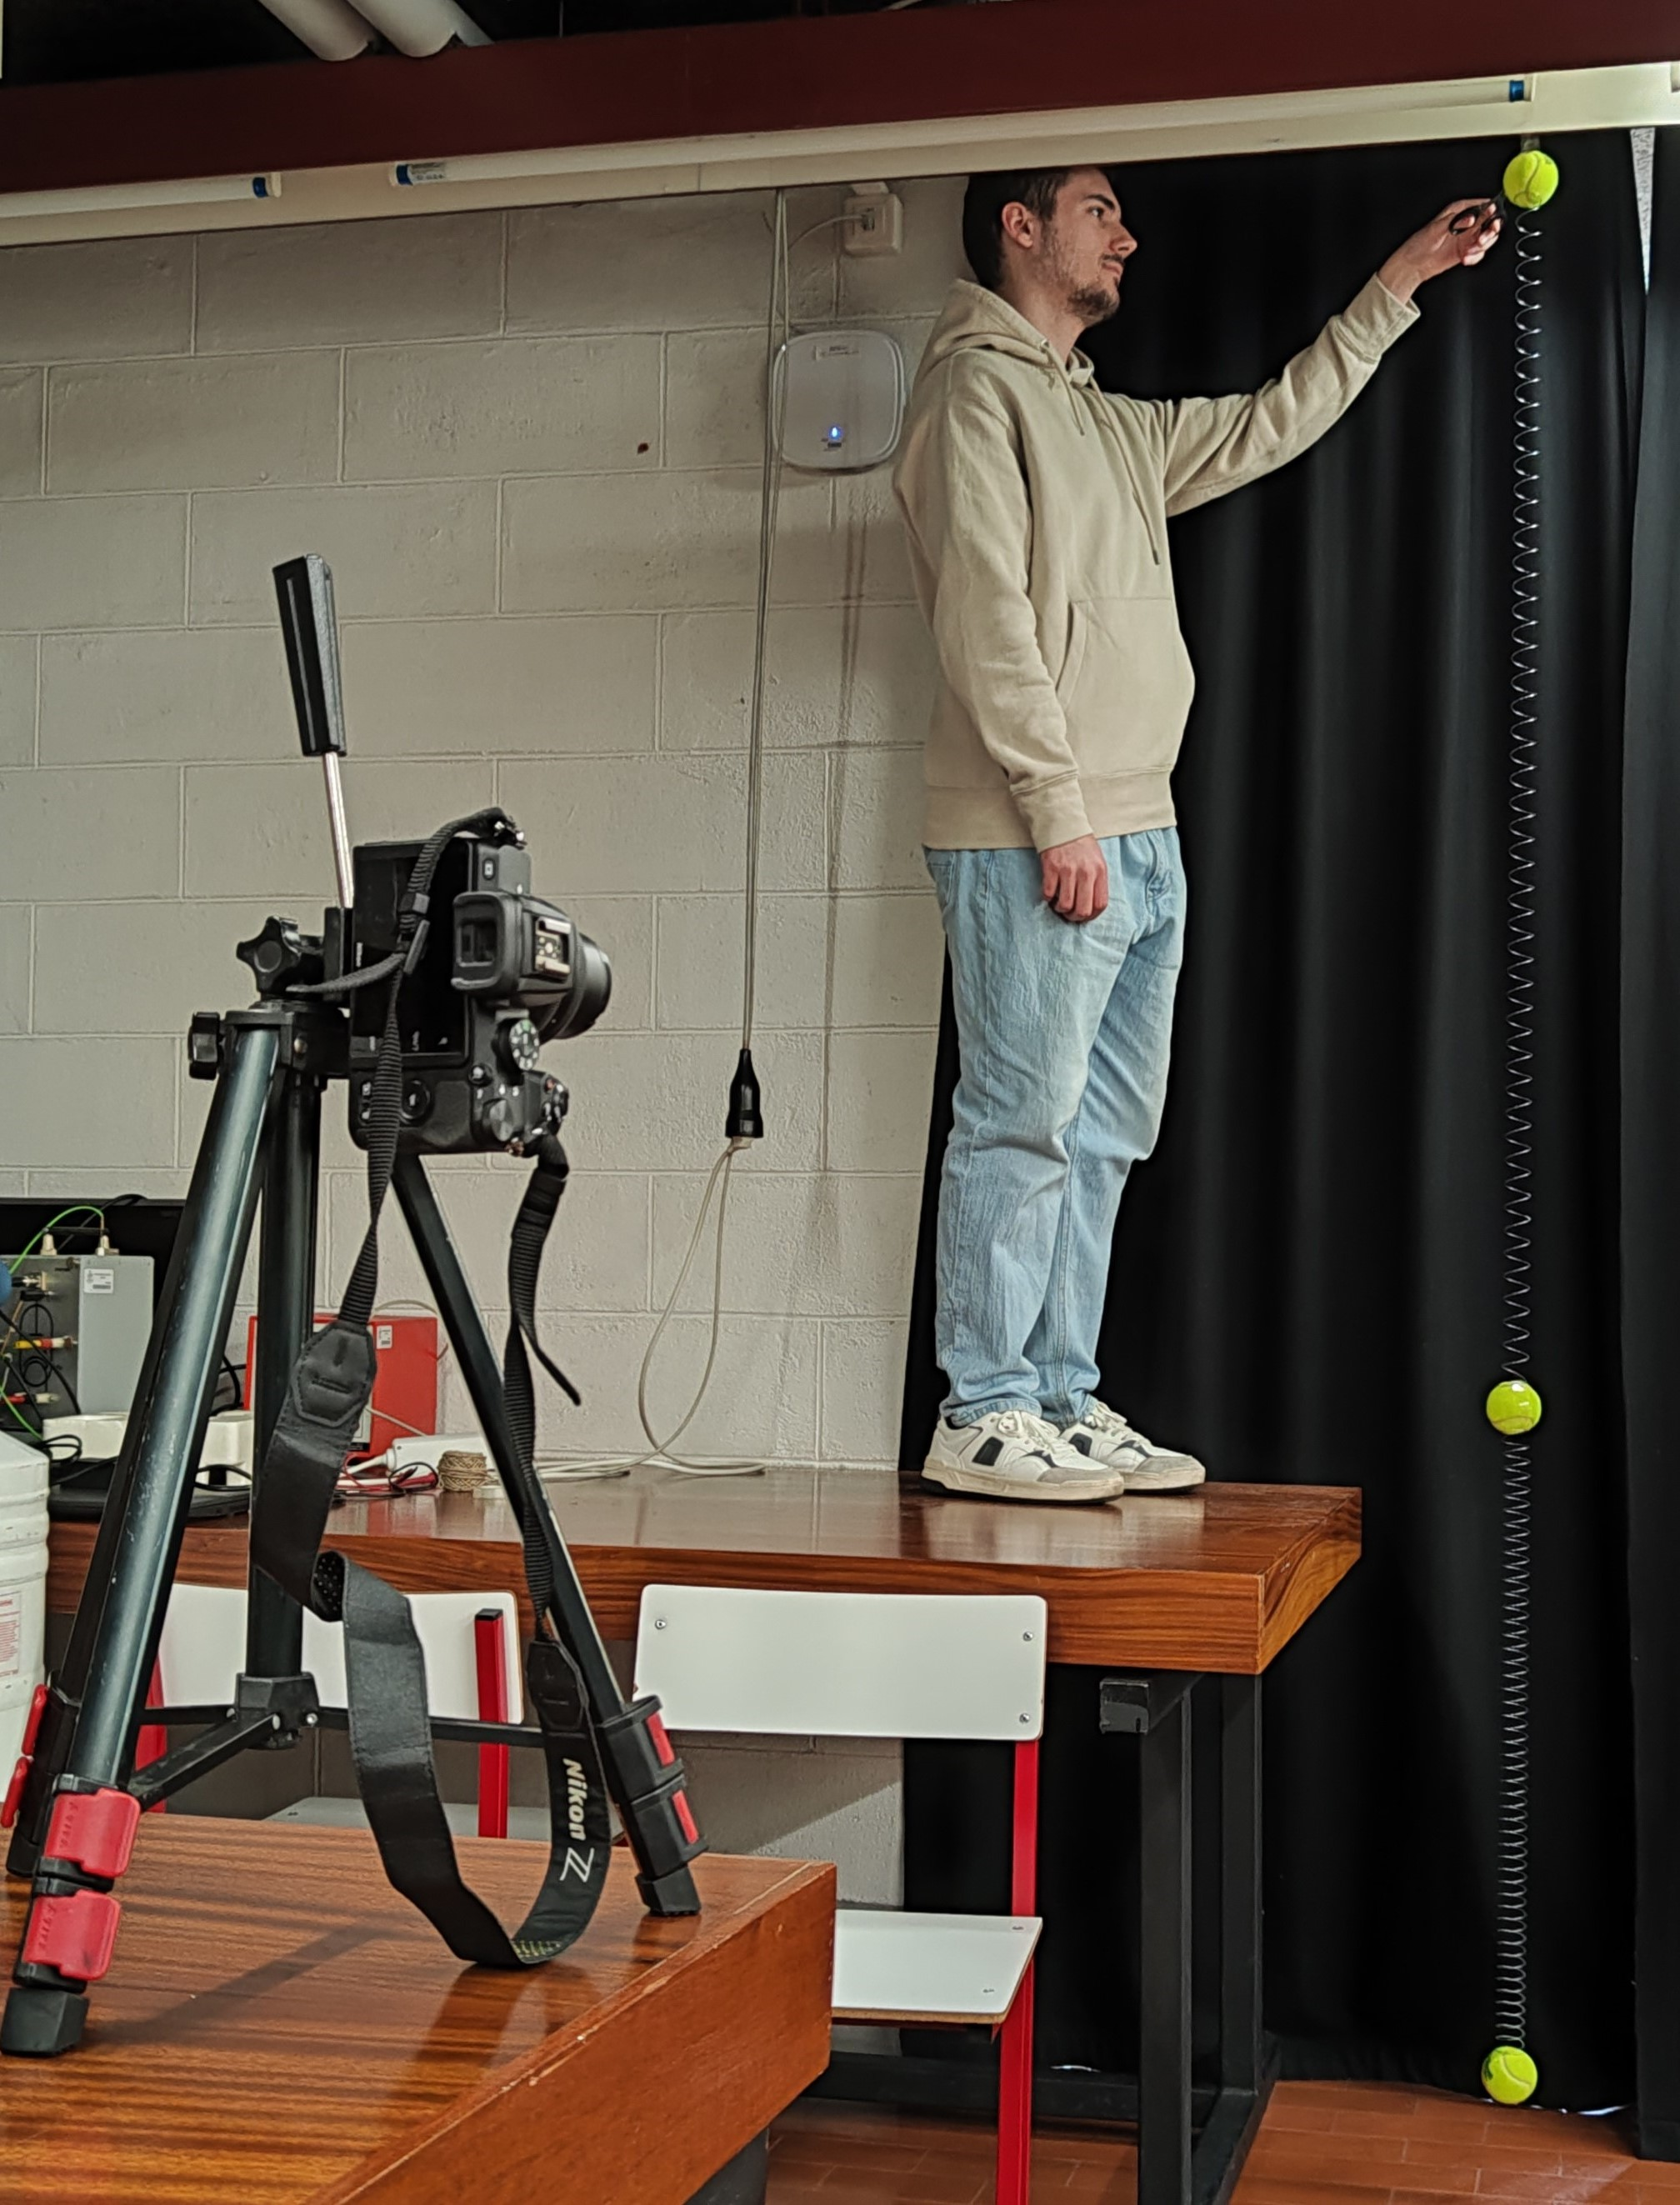
\includegraphics[height=20cm]{images/Final.jpg}
\caption{Procedimento usado para gravar a queda da bola.}
\end{figure}
\end{center}
\end{block}
\end{column}

\separatorcolumn
\begin{column}{\colwidth}
% -------------------------------
% Secção: Resultados
% -------------------------------
\begin{block}{Resultados}
Na Figura~\ref{fig:a}  estão representados gráficos da posição calculada e
observada de cada massas como funções do tempo, para os casos $N=2$ e $N=3$. É
patente o bom acordo entre os valores calculados e observados. As discrepâncias
mais significativas ocorrem no final do intervalo de tempo representado, quando
as espiras da mola se comprimem umas contra as outras, devido ao movimento de
queda mais rápido das massas mais acima, efeito que altera a dinâmica puramente
elástica e gravítica do modelo numérico.

É interessante notar a discrepância no movimento da massa na extremidade
da mola, mais patente no caso $N=2$ que para $N=3$. Cremos que esta discrepância
está relacionada com o modelo de mola ideal. Com apenas duas bolas de ténis
fixadas na mola, é mais discutível considerar-se desprezável a sua massa. Logo,
é mais expectável que o modelo adotado não se adeque tão precisamente ao
comportamento do sistema estudado.

Esta conjetura é apoiada por cálculos do valor da aceleração do centro de massa
do conjunto das bolas. O valor obtido a partir dos dados laboratoriais é
naturalmente inferior a $g$, uma vez que não inclui a contribuição do movimento
das molas. De facto, os valores obtidos são $8,27$\,m/s$^2$ para $N=2$ e
$9,11$\,m/s$^2$ para $N=3$.  A variação da discrepância nestes dois casos
sugere que se trata de uma função decrescente do número de bolas dispostas ao
longo da mola.  Ou seja, que a sua magnitude será tanto menor quanto menor for a
importância relativa da massa da mola; ou seja ainda, quanto mais ``ideal'' ela
for.
	
	\vspace{2cm}
	\begin{figure}
	\begin{tikzpicture}
			\begin{axis}[
			                %height=,
			                width=.4\colwidth,
			                domain=0:1,
			                xmin=0,xmax=.4,
			                xlabel=\textcolor{UBI}{tempo $(\unit{\second})$},
			                ymin=0,ymax=2.57,
			                scaled ticks = false,
			                %yticklabel style={/pgf/number format/.cd,fixed zerofill,precision=2},
			                ylabel=\textcolor{UBI}{Posição $(\unit{\metre})$},
					 ytick={0,0.5,1,1.5,2,2.5},yticklabels={0,0.5,1,1.5,2,2.5},
					 xtick={0,0.1,0.2,0.3,0.4},xticklabels={0,0.1,0.2,0.3,0.4},
			                %grid=both,major grid style={line width=.2pt,draw=#color},
			                %samples=#,
			                %every axis/.append style={axis line style={color}, tick style={color}},
			                legend style={draw=none},
			                legend cell align={left},
			                %legend pos= south west,
			                ticklabel style={UBI},
			                every axis/.append style={axis line style={UBI}, tick style={UBI}},
			                samples=800
			]
			\addplot[mypurple, smooth, thick] {-1621.92513511252*(x+0.055)^18 + 6121.49497805735*(x+0.055)^17 - 10620.203611305*(x+0.055)^16 + 11227.0136638144*(x+0.055)^15 - 8082.19566831113*(x+0.055)^14 + 4194.35994448389*(x+0.055)^13 - 1620.30359677421*(x+0.055)^12 + 474.390100098321*(x+0.055)^11 - 106.32394286827*(x+0.055)^10 + 18.1852651811809*(x+0.055)^9 - 1.45808049934885*(x+0.055)^8 + 0.232794509696558*(x+0.055)^7 - 3.30894854290934*(x+0.055)^6 + 0.000874488766885422*(x+0.055)^5 + 6.35364826832974*(x+0.055)^4 + 7.05060570450829e-7*(x+0.055)^3 - 9.81000000909166*(x+0.055)^2 - 1.32794452125934e-11*(x+0.055) + 2.53358200000001};
			\addlegendentry[UBI]{Massa $0$};
			\addplot[p6, smooth, thick] {1634.53401862378*(x+0.055)^18 - 6167.3076951656*(x+0.055)^17 + 10696.4801165736*(x+0.055)^16 - 11304.1277205007*(x+0.055)^15 + 8135.07552593306*(x+0.055)^14 - 4220.38221968951*(x+0.055)^13 + 1629.78555495354*(x+0.055)^12 - 476.992106082573*(x+0.055)^11 + 106.86554864998*(x+0.055)^10 - 18.2707144835056*(x+0.055)^9 + 1.46821509336611*(x+0.055)^8 - 0.233683127949648*(x+0.055)^7 + 3.30900455585977*(x+0.055)^6 - 0.000876914247492155*(x+0.055)^5 - 6.35364820157578*(x+0.055)^4 - 7.06060625657539e-7*(x+0.055)^3 + 9.09672372349551e-9*(x+0.055)^2 + 1.32985411272606e-11*(x+0.055) + 0.659303499999993};
			\addlegendentry[UBI]{Massa $1$};
			\addplot[mydeeppurple,loosely dotted, line width=1mm] table[x = t, y = X1] {Lab.dat};
			\addplot[p5, loosely dotted, line width=1mm] table[x = t, y = X2] {Lab.dat};
			
			\end{axis}
		\end{tikzpicture}
		\begin{tikzpicture}
			\begin{axis}[
			%height=,
			width=.4\colwidth,
			domain=0:0.5,
			xmin=0,
			xmax=0.38,
			legend style={fill=white,draw=none},
			legend cell align={left},
			%legend pos=outer north east,
			xlabel=\textcolor{UBI}{tempo $(\unit{\second})$},
			ytick={0,0.5,1,1.5,2,2.5},yticklabels={0,0.5,1,1.5,2,2.5},
			xtick={0,0.1,0.2,0.3,0.4},xticklabels={0,0.1,0.2,0.3,0.4},
			ymax=2.57,
			ymin=0,
			ylabel=\textcolor{UBI}{Posição $(\unit{\metre})$},
			%grid=both,
			%major grid style={line width=.2pt,draw=pag!95},
			samples=400,
			%ticks=none,
			%ylabel=,
			ticklabel style={UBI},
			every axis/.append style={axis line style={UBI}, tick style={UBI}}
			]	
			\addplot[mylime, smooth, thick] {+2.4508266637798486+1.92551978e-06-7.08288771e-04*x-1.46868493e+01*x^2-4.09976421e-01*x^3+2.18585827e+01*x^4-9.39435949e+00*x^5-6.34499469e+00*x^6};
			\addlegendentry[UBI]{Massa 0}	
			\addplot[mypurple, smooth, thick] {0.9655805946162642+5.849073753628633*x^6+16.602620664621227*x^5-23.992790391059497*x^4+0.721408292027056*x^3-0.049464418381870844*x^2+0.0012431133324992847*x-3.3748416628826994e-06};
			\addlegendentry[UBI]{Massa 1}
			\addplot[p6, smooth, thick] {0.12706810953816955+0.49592093161308015*x^6-7.2082611722205305*x^5+2.1342076920531725*x^4-0.311431870599336*x^3+0.02131369465598449*x^2-0.0005348245618400737*x+1.449321886986526e-06};
			\addlegendentry[UBI]{Massa 2}	
			%%%%%%%%%%%%%%%%%%%%%%%%%%%%%%%%Laboratoriais%%%%%%%%%%%%%%%%%%%%%%%%%%%%%%%%%%%%%%%%%%%%%%%%%%%%
			\addplot[mylightgreen, loosely dotted, line width=1mm] 						{2.45082666-5.52077707e-01*(x+0.05)+3.43475522e+01*(x+0.05)^2-7.74480255e+02*(x+0.05)^3+7.67559430e+03*(x+0.05)^4-4.78466157e+04*(x+0.05)^5+1.85156584e+05*(x+0.05)^6-4.25893494e+05*(x+0.05)^7+5.29402858e+05*(x+0.05)^8-2.72302397e+05*(x+0.05)^9};
			\addplot[mydeeppurple,loosely dotted, line width=1mm] {+236878.24663477603*(x+0.05)^9-445940.6935199308*(x+0.05)^8+341684.85624595085*(x+0.05)^7-137516.49356955112*(x+0.05)^6+31308.952389044767*(x+0.05)^5-4064.7449218401653*(x+0.05)^4+286.3968820830498*(x+0.05)^3-9.702864113503072*(x+0.05)^2+0.14861681786073874*(x+0.05)+0.9655805946162642};
			\addplot[p5, loosely dotted, line width=1mm] {+5919.067897122547*(x+0.05)^9-11617.379837153167*(x+0.05)^8+9381.76346394042*(x+0.05)^7-4036.0015719443286*(x+0.05)^6+992.5740054163633*(x+0.05)^5-138.15718216106012*(x+0.05)^4+9.591644806308794*(x+0.05)^3-0.1774404113040594*(x+0.05)^2+0.019261796302454434*(x+0.05)+0.12706810953816955};        
			\end{axis}
		\end{tikzpicture}
		\caption{\label{fig:a} Deslocamentos das massas na queda de uma mola com 2 e 3 massas. A tracejado estão as curvas observadas e a contínuo estão as soluções numéricas.}
	\end{figure}
	\vspace{2cm}
Na Figura~\ref{fig:b} está representada a posição da massa na extremidade inferior da
mola, como função do tempo, para diferentes números (2, 3, 4 e 5) de massas
dispostas na mola. Nota-se quanto maior for o número de massas, maior é o
atraso no início do movimento da última massa. Este facto sugere que o
comportamento de queda das molas demonstrado nos vídeos referidos resulta da
densidade de massa finita das molas reais.
\vspace{2cm}
	\begin{figure}
		\begin{tikzpicture}
			\begin{axis}[
			                %height=,
			                width=.4\colwidth,
			                % domain=52:60,
			                xmin=0,xmax=.4,
			                xlabel=\textcolor{UBI}{tempo $(\unit{\second})$},
			               % ticks=none,
			                xtick={0,0.1,0.2,0.3,0.4},xticklabels={0,0.1,0.2,0.3,0.4},
			                ymin=-0.05,ymax=0.01,
			                scaled ticks = false,
			                %yticklabel style={/pgf/number format/.cd,fixed zerofill,precision=2},
			                ylabel=\textcolor{UBI}{Posição $(\unit{\centi\metre})$},
		                       ytick={-0.05,-0.03,-0.01,0.01},yticklabels={-5,-3,-1,1},
			                %grid=both,major grid style={line width=.2pt,draw=#color},
			                %samples=#,
			                %every axis/.append style={axis line style={color}, tick style={color}},
			                legend style={draw=none},
			                legend cell align={left},
			                legend pos= south west,
			                ticklabel style={UBI},
			                every axis/.append style={axis line style={UBI}, tick style={UBI}}
			]
			\addplot[p5, thick] table[x = T, y = X1] {1.dat};
			\addlegendentry[UBI]{$N=2$};
			\addplot[p6, thick] table[x = T, y = X2] {1.dat};
			\addlegendentry[UBI]{$N=3$};
			\addplot[p7, thick] table[x = T, y = X3] {1.dat};
			\addlegendentry[UBI]{$N=4$};
			\addplot[p8, thick] table[x = T, y = X4] {1.dat};
			\addlegendentry[UBI]{$N=5$};
			\end{axis}
		\end{tikzpicture}
		\caption{\label{fig:b} Posição da massa na extremidade inferior da mola, em função do tempo, para diferentes valores de $N$.}
	\end{figure}
	\vspace{2cm}
\end{block}
% -------------------------------
% Secção: Conclusões
% -------------------------------
\begin{exampleblock}{Conclusões}

O movimento de queda de molas elásticas reais ilustrado nos vídeos referidos na
Introdução pode ser descrito aproximadamente usando um modelo de mola ideal com
massas pontuais dispostas regularmente ao longo do seu comprimento, apesar de
ser uma manifestação do caráter contínuo da distribuição de massa das molas
elásticas usadas nas demonstrações. Estas massas são indispensáveis para dotar o
modelo de mola ideal com peso e inércia e, assim, promover as molas ideais ao
estatuto de objetos dinâmicos.

A descrição do movimento torna-se mais exata quanto maior for o número de massas
pontuais considerada, o que concorda com a ideia de uma mola real como limite
contínuo de uma mola ideal com massas pontuais distribuídas ao longo do seu
comprimento. 

Todos os ficheiros produzidos neste trabalho (vídeos, ficheiros de dados, programas) estão disponíveis em \url{https://github.com/ljmamoreira/fslinky} (acesso possível também pelo QR code abaixo).

%Este problema (com a abordagem que propomos) parece-nos um contexto adequado para
%a ilustração das teorias de campo como limites continuos de teorias de massas
%pontuais.
\end{exampleblock}
% -------------------------------
% Secção: Referências
% -------------------------------
%\begin{block}{Referências}
%\begin{multicols}{2}
%    \footnotesize
%    \bibliographystyle{plainurl}
%    \bibliography{poster}
%\end{multicols}
%%    \nocite{*}
%%    \footnotesize{\bibliographystyle{plainurl}\bibliography{poster}}
%\end{block}
% -------------------------------
% Section: Portfolio
% -------------------------------
%\begin{block}{Mais Informações}
%    \begin{figure}[h]
    \centering
    
\includegraphics[height=8cm]{images/qrcode2.png}
    \label{fig:figure3}
\end{figure}
%\end{block}
\end{column}
\separatorcolumn
\end{columns}
%\separatorcolumn
\begin{columns}[t]
\begin{column}{0.9328981723\paperwidth}
\begin{block}{Referências}
\begin{multicols}{2}
\begin{multicols}{3}
    \nocite{*}
    \scriptsize
    \bibliographystyle{unsrturl}
    \bibliography{poster}
\end{multicols}
    \hfill
    \begin{figure}
    \centering
  \vspace*{-1.45cm}\hfill
\includegraphics[height=8cm]{images/qrcode2}
\end{figure}
%    \begin{figure}[h]
    \centering
    
\includegraphics[height=8cm]{images/qrcode2.png}
    \label{fig:figure3}
\end{figure}
\end{multicols}
\end{block}
\end{column}
\end{columns}
\end{frame}
\end{document}
